\section{Simulaciones y barrido del espacio de parámetros}
Para lograr un equilibrio entre coste computacional y precisión, se ha optado por utilizar
el algoritmo de Runge-Kutta de cuarto orden (RK4), implementando un paso de 
tiempo adaptativo, gobernado por los siguientes parámetros:
\begin{itemize}
    \item \texttt{total\_t}: El tiempo total de simulación.
    Este periodo debe ser suficiente para abarcar toda la trayectoria de transferencia desde el lanzamiento 
    hasta un posible encuentro con Venus.
    \item \texttt{factor}, $f$: Factor de tolerancia multiplicativo. 
    Este parámetro se fija de manera arbitraria, y multiplicará a la fórmula del cáclulo de $dt$.
    \item \texttt{precision\_factor}, $p_f$: Factor divisor de precisión. 
    Cuando la nave se acerque a una distancia crítica, que se ha fijado
    de forma completamente arbitraria en $10^6\text{ km}$, el paso temporal $dt$ se divide por 
    este factor para simular correctamente la violenta variación de energía sufrida en la asistencia gravitatoria
    \footnote{Esto supone una pequeña discontinuidad en la energía, lo que se ve reflejado en las gráficas
    de energía; sin embargo, esta variación es del orden de magnitud de la variación total a lo largo de toda la simulación;
    del orden de $10^{-14}$}.
    \item \texttt{max\_dt}, $M_{dt}$, y \texttt{min\_dt}, $m_{dt}$: Los topes superior e 
    inferior del paso de tiempo (expresados en segundos). Permiten que la simulación 
    avance rápidamente cuando no es necesaria una precisión extrema, y evitan que la simulación 
    quede bloqueada intentando conseguir una precisión infinita cuando la distancia es muy pequeña.
\end{itemize}
Con todo, el valor de \texttt{dt} se calculará utilizando la siguiente expresión:
$$
dt = f \cdot \sqrt[3]{r_v}
$$
Donde $r_v$ es la distancia a Venus de la nave.
Además, nos podemos encontrar con las siguientes casuísticas:
Además, se pueden encontrar las siguientes casuísticas:
\begin{itemize}
    \item Si $dt > M_{dt}$, se asigna $dt = M_{dt}$.
    \item Si $dt < m_{dt}$, se asigna $dt = m_{dt}$.
    \item Si $r_v < 10^9\text{ m}$, se asigna $dt = \dfrac{dt}{p_f}$ (es decir, se divide por \texttt{precision\_factor}).
\end{itemize}

\subsection{Primera aproximación}
En primer lugar, con el objetivo de realizar una exploración inicial del espacio de parámetros, 
se ha planteado un barrido grueso de 65341 simulaciones, para barrer el espacio cada $1^\circ$ de cada grado de libertad. 
Dado el elevado número de ejecuciones, se ha optado por relajar la precisión del integrador numérico para acelerar 
los cálculos, pero sin comprometer significativamente la validez física del sistema.
De este modo, los parámetros de inicialización del código utilizados para esta primera aproximación son:

\bigskip
\noindent\begin{minipage}{0.5\textwidth}\scriptsize
\begin{verbatim}
double min_yaw_angle = -180.0;
double max_yaw_angle = 180.0;
double min_pitch_angle = -90.0;
double max_pitch_angle = 90.0;
double total_t = 400.0;
double factor = 0.1;
\end{verbatim}
\end{minipage}%
\begin{minipage}{0.5\textwidth}\scriptsize
\begin{verbatim}
double precision_factor = 10.0;
double max_dt = 100;
double min_dt = 0.1;
int pitch_sims = 181;
int yaw_sims = 361;
int total_sims = yaw_sims*pitch_sims;
\end{verbatim}
\end{minipage}

\bigskip

Se obtiene así el siguiente gráfico:
\begin{figure}[H]
    \centering
    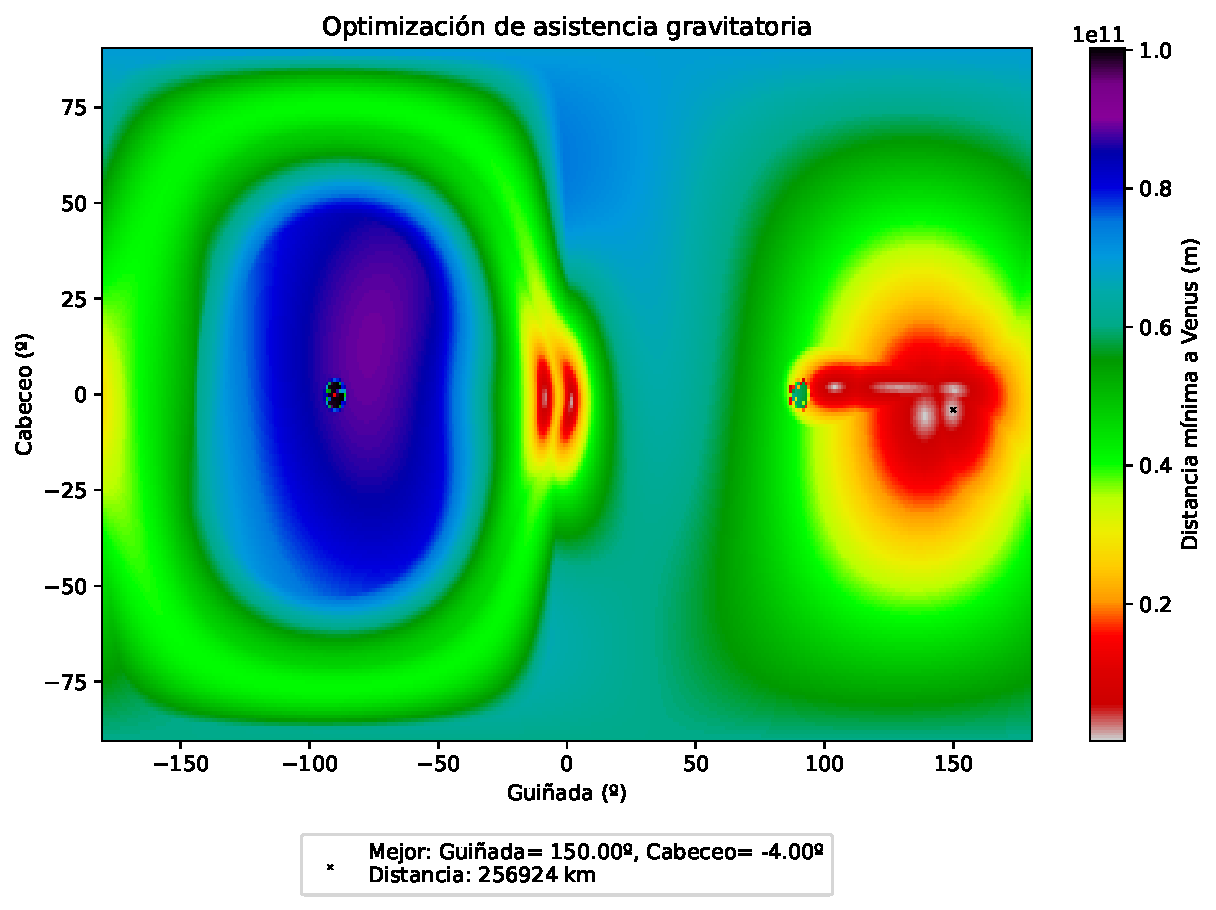
\includegraphics[width=\textwidth]{graphs/heatmap_20260616_162424.pdf}
    % \caption{Mapa de calor que muestra la distancia mínima a Venus en función del ángulo de guiñada y cabeceo.}
\end{figure}
\vspace{-0.5cm}
En él, se pueden apreciar dos principales focos donde la distancia a Venus es pequeña en relación con el resto, 
lo que, como ya ha sido dicho, se corresponde con una mayor transferencia de energía entre Venus y la Nave.
Además, también se pueden observar dos puntos donde ocurren fenómenos extraños; el correspondiente a 
$\sim -100^\circ$ es un choque con la Tierra, y el de $\sim 100^\circ$ con el Sol.
\subsection{Exploración del primer foco}
El primer foco se encuentra ubicado en un entorno de los $0^\circ$ tanto de guiñada como de cabeceo y,
dado que estos valores se corresponden con una velocidad inicial que apunta en la dirección de la de la 
Tierra, se comienza explorando esta zona.
Se realiza entonces un barrido de ángulo de guiñada comprendido en el intervalo $[-20^\circ, +10^\circ]$ y de cabeceo
en $[-15^\circ, +15^\circ]$, con una resolución de $0.25^\circ$. Los parámetros para esta fase son:

\bigskip
\noindent\begin{minipage}{0.5\textwidth}\scriptsize
\begin{verbatim}
double min_yaw_angle = -20.0;
double max_yaw_angle = 10.0;
double min_pitch_angle = -15.0;
double max_pitch_angle = 15.0;
double total_t = 400.0;
double factor = 0.05;
\end{verbatim}
\end{minipage}%
\begin{minipage}{0.5\textwidth}\scriptsize
\begin{verbatim}
double precision_factor = 50.0;
double max_dt = 100;
double min_dt = 0.05;
int pitch_sims = 121;
int yaw_sims = 121;
int total_sims = yaw_sims*pitch_sims;
\end{verbatim}
\end{minipage}

\bigskip

Se obtiene el siguiente gráfico:
\begin{figure}[H]
    \centering
    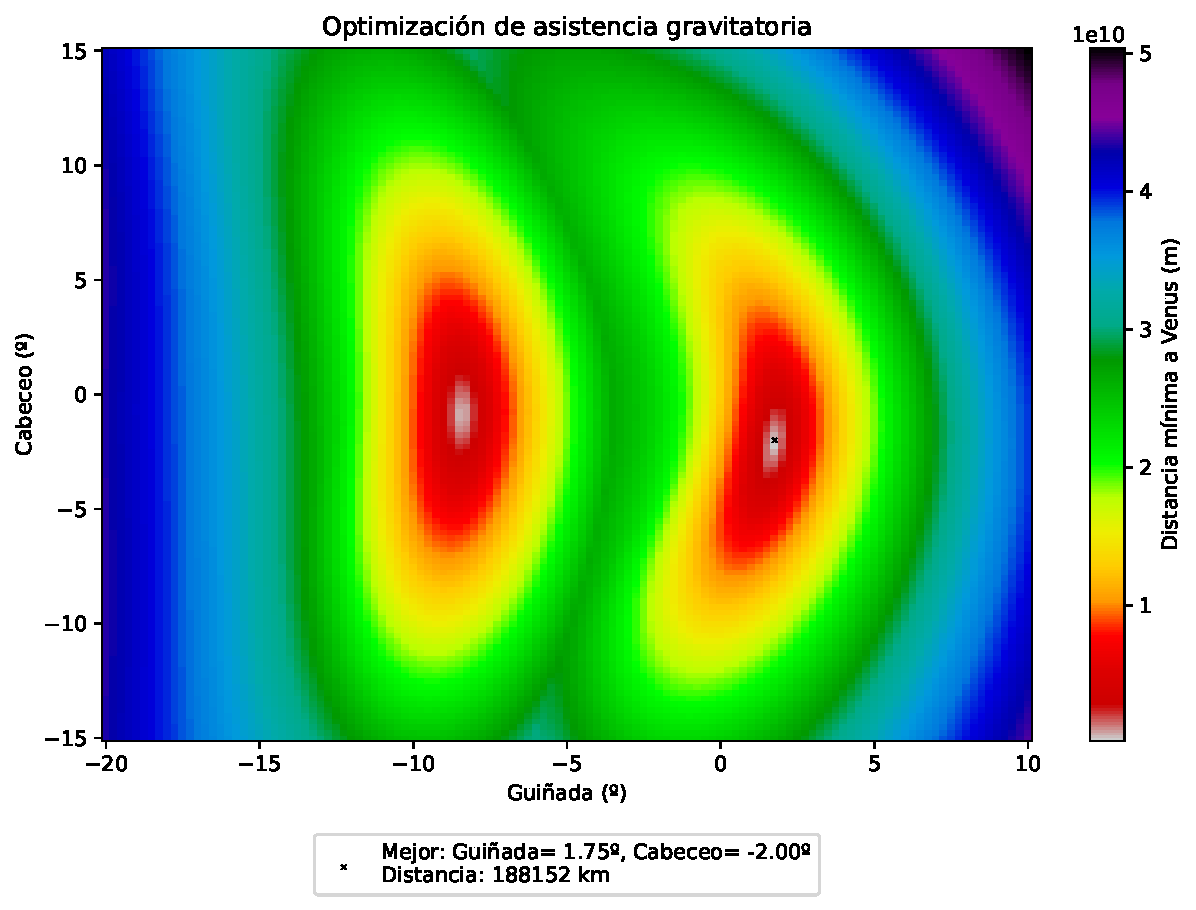
\includegraphics[width=\textwidth]{graphs/heatmap_20260616_164711.pdf}
\end{figure}
Para hilar incluso más fino, se realizará a continuación un análisis centrado en cada una de las dos ventanas:


\subsubsection{Primera ventana}
En primer lugar, se estudia la ventana izquierda, con una resolución de $0.05^\circ$:

\bigskip
\noindent\begin{minipage}{0.5\textwidth}\scriptsize
\begin{verbatim}
double min_yaw_angle = -10.0;
double max_yaw_angle = -6.0;
double min_pitch_angle = -4.0;
double max_pitch_angle = 2.5;
double total_t = 400.0;
double factor = 0.05;
\end{verbatim}
\end{minipage}%
\begin{minipage}{0.5\textwidth}\scriptsize
\begin{verbatim}
double precision_factor = 50.0;
double max_dt = 50;
double min_dt = 0.01;
int pitch_sims = 131;
int yaw_sims = 81;
int total_sims = yaw_sims*pitch_sims;
\end{verbatim}
\end{minipage}

\bigskip

Se obtiene el siguiente resultado:
\begin{figure}[H]
    \centering
    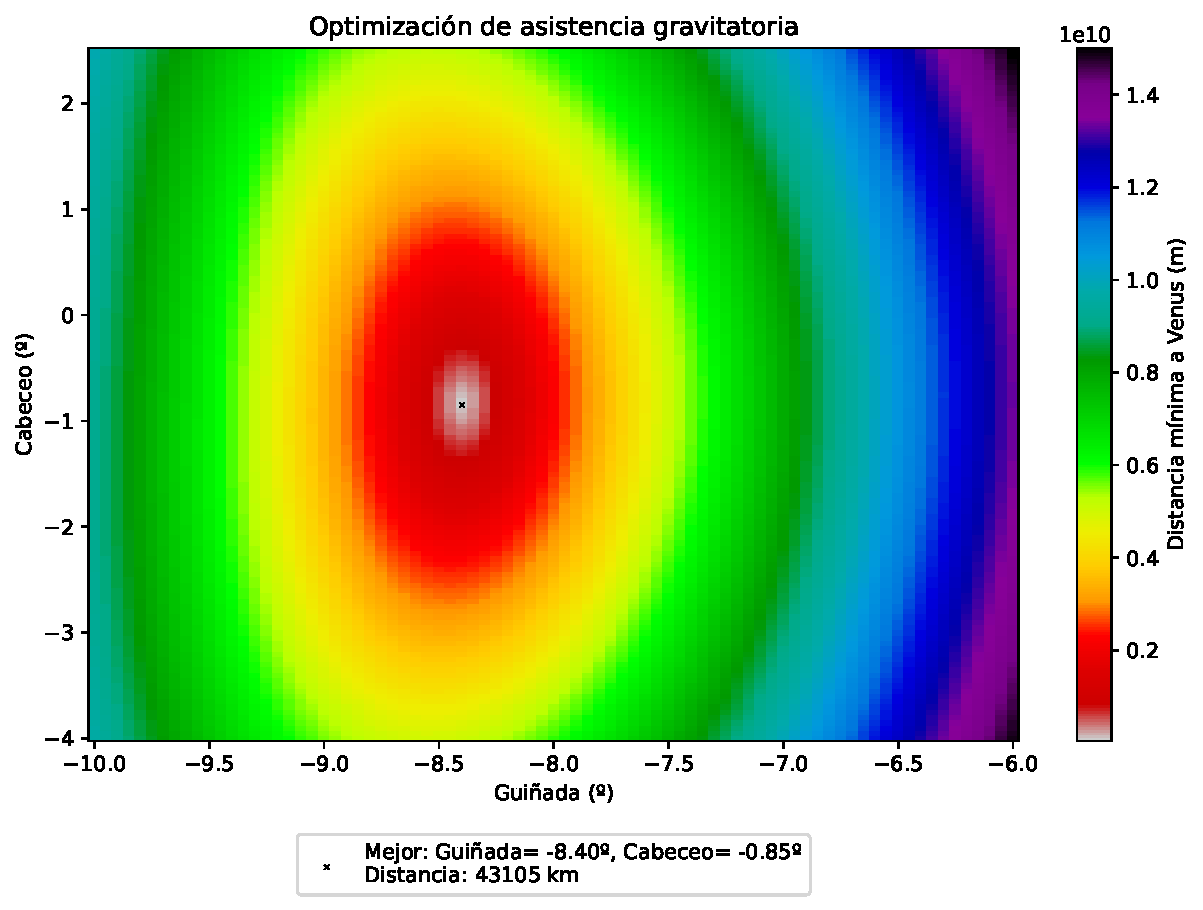
\includegraphics[width=\textwidth]{graphs/heatmap_20260616_170902.pdf}
\end{figure}

Finalmente, para localizar el mínimo con la máxima precisión posible, se realiza un último barrido 
sobre la ventana izquierda, entre $-9^\circ$ y $-8^\circ$ de guiñada y 
entre $-1^\circ$ y $0^\circ$ de cabeceo. 
La resolución se aumenta a $0.005^\circ$, lo que equivale a $18$ segundos de arco. 
Esta configuración resulta en 40401 simulaciones, un número exigente pero asumible.
\newpage
Los parámetros para esta fase final son:

\bigskip
\noindent\begin{minipage}{0.5\textwidth}\scriptsize
\begin{verbatim}
double min_yaw_angle = -9.0;
double max_yaw_angle = -8.0;
double min_pitch_angle = -1.0;
double max_pitch_angle = 0.0;
double total_t = 400.0;
double factor = 0.05;
\end{verbatim}
\end{minipage}%
\begin{minipage}{0.5\textwidth}\scriptsize
\begin{verbatim}
double precision_factor = 50.0;
double max_dt = 50;
double min_dt = 0.01;
int pitch_sims = 201;
int yaw_sims = 201;
int total_sims = yaw_sims*pitch_sims;
\end{verbatim}
\end{minipage}

\bigskip

\begin{figure}[H]
    \centering
    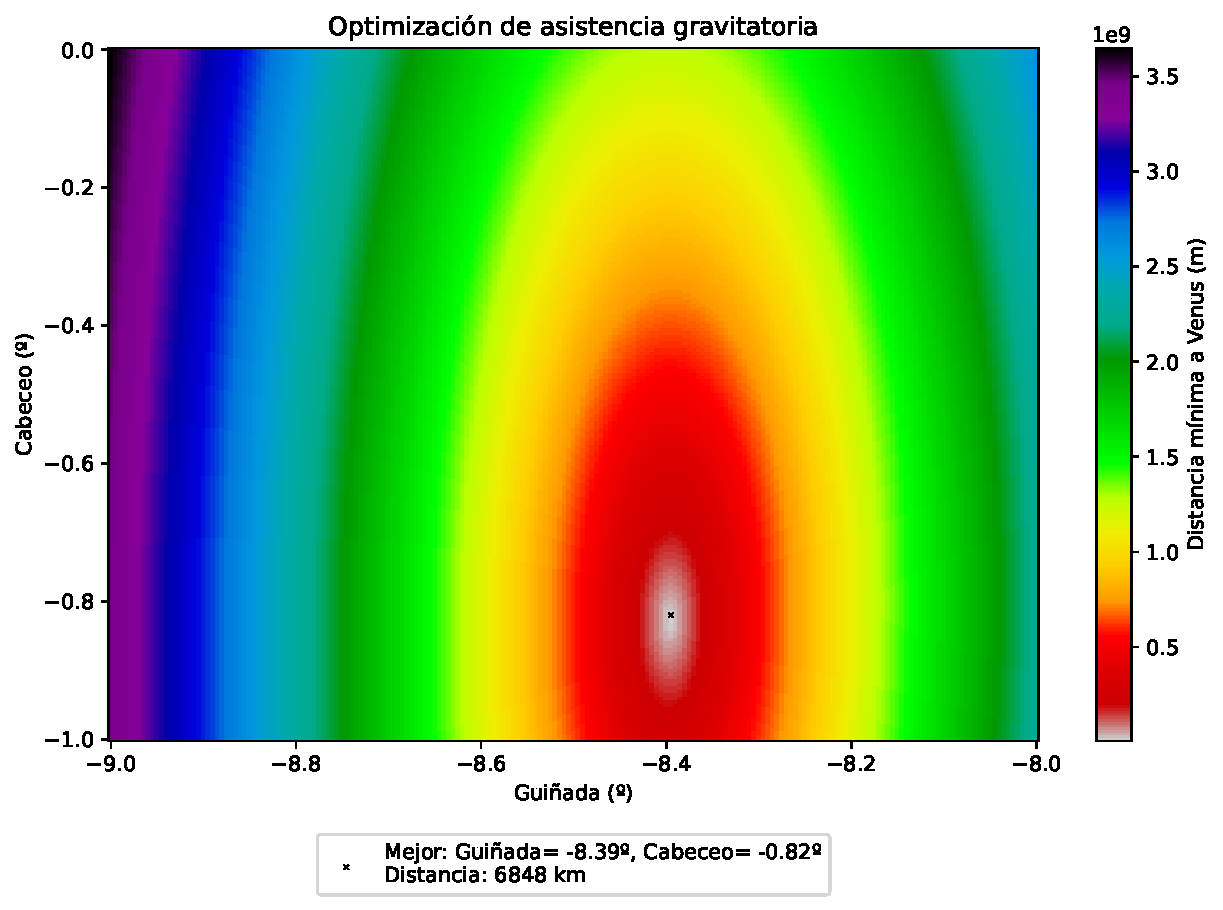
\includegraphics[width=\textwidth]{graphs/heatmap_20260616_181013.pdf}
\end{figure}
Los ángulos óptimos obtenidos son:
\begin{itemize}
    \item Guiñada, $\varphi = -8.39500^\circ$
    \item Cabeceo, $\theta = -0.82000^\circ$
\end{itemize}


\newpage
\subsubsection{Segunda ventana}
A continuación, se explora la segunda ventana de interés, con una resolución de $0.05^\circ$. El barrido se realiza en el intervalo de guiñada $[0^\circ, 4^\circ]$ y de cabeceo $[-4.5^\circ, 2^\circ]$.
Los parámetros para esta fase son:

\bigskip
\noindent\begin{minipage}{0.5\textwidth}\scriptsize
\begin{verbatim}
double min_yaw_angle = 0.0;
double max_yaw_angle = 4.0;
double min_pitch_angle = -4.5;
double max_pitch_angle = 2.0;
double total_t = 400.0;
double factor = 0.05;
\end{verbatim}
\end{minipage}%
\begin{minipage}{0.5\textwidth}\scriptsize
\begin{verbatim}
double precision_factor = 50.0;
double max_dt = 50;
double min_dt = 0.01;
int pitch_sims = 131;
int yaw_sims = 81;
int total_sims = yaw_sims*pitch_sims;
\end{verbatim}
\end{minipage}

\bigskip

\begin{figure}[H]
    \centering
    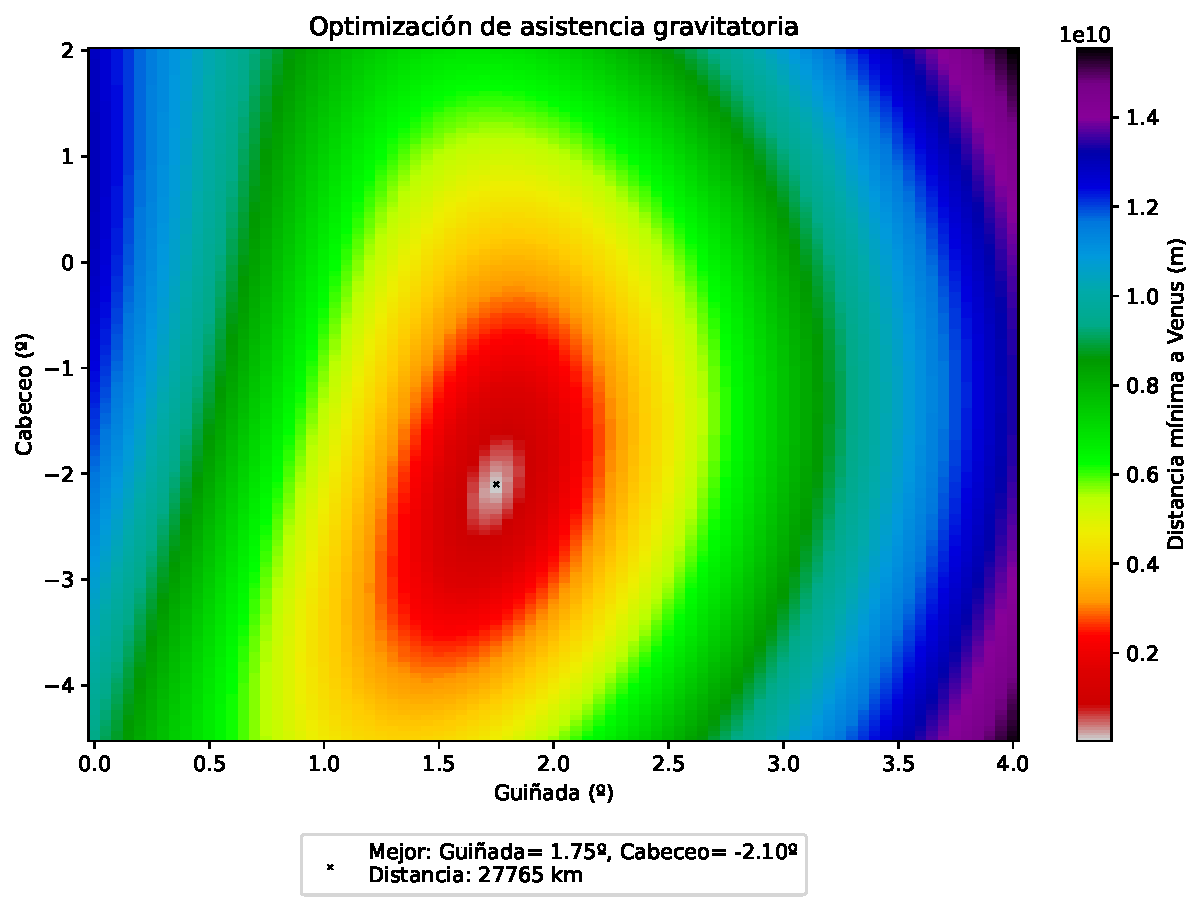
\includegraphics[width=\textwidth]{graphs/heatmap_20260616_182644.pdf}
\end{figure}


\bigskip

De nuevo, para localizar el mínimo con la máxima precisión posible, se realiza un último barrido 
sobre esta segunda ventana, entre $1.5^\circ$ y $2^\circ$ de guiñada y 
entre $-2.3^\circ$ y $-1.8^\circ$ de cabeceo. 
La resolución se mantiene en $0.005^\circ$ (18 segundos de arco). 
Esta configuración resulta en 10201 simulaciones.
\newpage
Los parámetros para esta fase final son:

\bigskip
\noindent\begin{minipage}{0.5\textwidth}\scriptsize
\begin{verbatim}
double min_yaw_angle = 1.5;
double max_yaw_angle = 2.0;
double min_pitch_angle = -2.3;
double max_pitch_angle = -1.8;
double total_t = 400.0;
double factor = 0.05;
\end{verbatim}
\end{minipage}%
\begin{minipage}{0.5\textwidth}\scriptsize
\begin{verbatim}
double precision_factor = 50.0;
double max_dt = 50;
double min_dt = 0.01;
int pitch_sims = 101;
int yaw_sims = 101;
int total_sims = yaw_sims*pitch_sims;
\end{verbatim}
\end{minipage}
\bigskip

\begin{figure}[H]
    \centering
    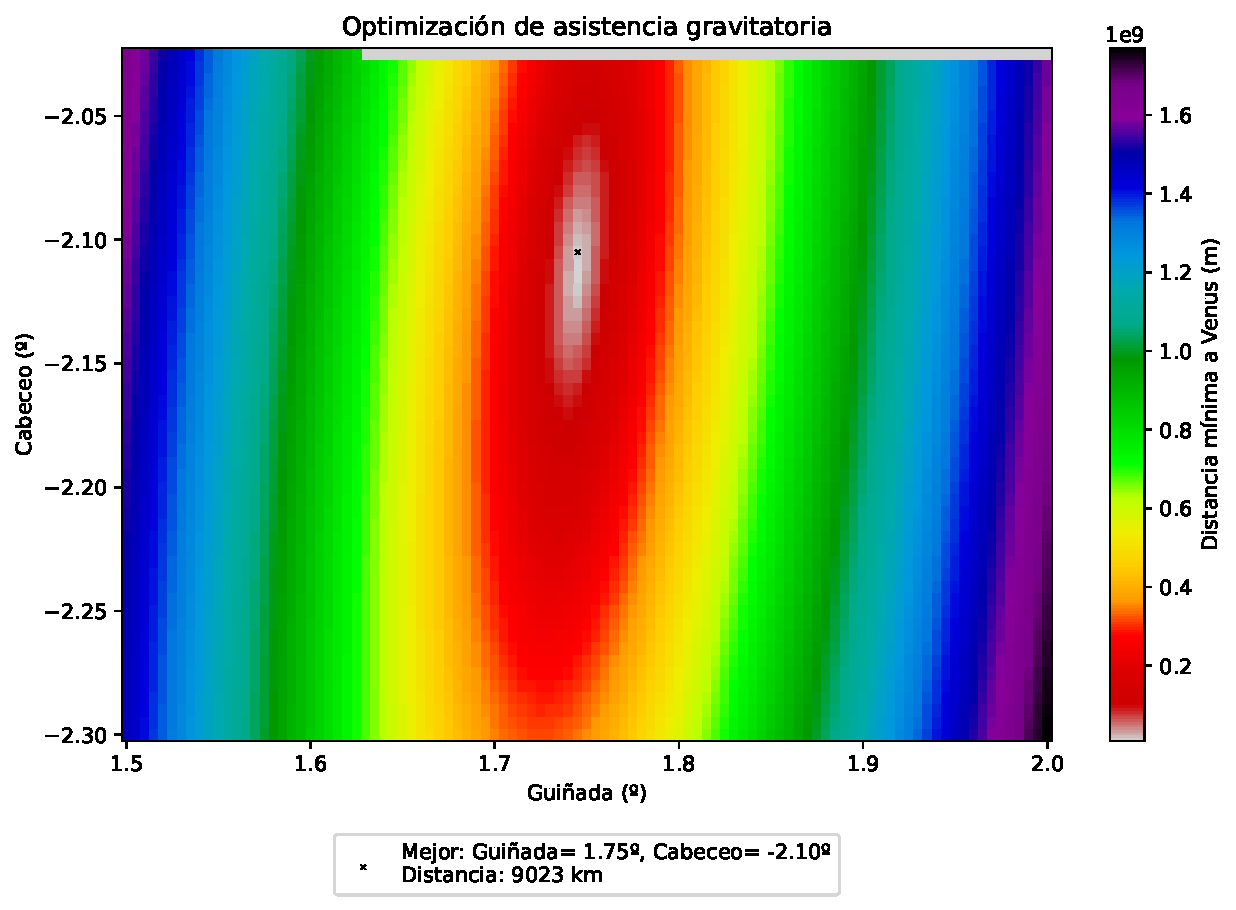
\includegraphics[width=\textwidth]{graphs/heatmap_20260616_184803.pdf}
\end{figure}
Los ángulos óptimos obtenidos son:
\begin{itemize}
    \item Guiñada, $\varphi = 1.74500^\circ$
    \item Cabeceo, $\theta = -2.10500^\circ$
\end{itemize}